\chapter{The Radiative Quenching \texorpdfstring{$ H_2^+ $}{$H_2^+$}  Ion Atom Collisions in 2D Space} 
\label{chp:quenching}

The analysis of the radiative processes is related to the analysis of the general scattering process. So we list those.

Typically for the scattering processes at this level, we can distinguish between the radiative and non-radiative processes. 

Radiative processes involve emission of a photon and they typically mean Radiative Charge Transfer: \\
$ A(n+1\prescript{1}{}S) + B \longleftrightarrow A(n\prescript{1}{}S) + B + \hbar\omega $ \\
and Radiative Association: \\
$ A(n+1\prescript{1}{}S) + B \longleftrightarrow A(n\prescript{1}{}S)B + \hbar\omega $ .\\
For example, the simplest case of the radiative process is the collision of the two hydrogen atoms, in the process $ H + H^+ \rightarrow H^+ + H + \hbar\omega $.\\

While the non-radiative process, with no photon emission, is a Charge Transfer: \\
$ A(n+1\prescript{1}{}S) + B(n\prescript{1}{}S) \longleftrightarrow  A(n\prescript{1}{}S) + B(n+1\prescript{1}{}S) $ .\\

Radiative Quenching is an interaction between two atoms (or molecules), one being in excited state and the other in 'normal' ground state. During this process the excited atom emits a photon and drops to a ground state.
The simplest such case is the collision of the two hydrogen molecules, in the process $ H_2(2\,{}^2\!S) + H_2(1\,{}^2\!S) \rightarrow H_2(1\,{}^2\!S) + H_2(1\,{}^2\!S) + \hbar\omega $.

There are several theoretical approaches to this problem. \cite{RadQuench1}, \cite{RadQuench2}, \cite{Zygelman88}. While the problem has not been solved analytically, we will show that it can be solved numerically, to a desired precision. The radiative processes are driven by the interaction of the collision system with the radiation field. The direct change transfer is due to the transition between atomic (molecular) states due to the nuclear motion. Because the collision energy considered is low, typically only molecular states included are those which correspond to the initial $ A \prescript{1}{}\Sigma^+ $  and final $ X \prescript{1}{}\Sigma^+ $ channels.

Here we shall investigate the low energy collision process between the hydrogen atom and the hydrogen ion, in 2 dimension. We use fully quantum mechanical approach to calculate the cross section and the emission spectra of the reaction $ H(2\prescript{2}{}S) + H(1\prescript{1}{}S)\rightarrow H(1\prescript{1}{}S) + H(1\prescript{1}{}S) + \hbar\omega $, formed by the quenching of the excited $ H $ atom by the approaching $ H $ atom, in 2D dimensions. To my knowledge, there is no experimental results related to the 2D problem. There are results for the 3D case, listed in \cite{Zygelman88} and references there.

In this calculation, the atoms are confined in 2 dimensions, while the radiation is emitted or absorbed in all 3D space. Therefore the photon can be emitted in any direction and the potential felt by the incoming ion is the standard 3D Coulomb potential.

We will model this as a scattering problem, using a Born-Oppenheimer approximation and optical theorem. The Hamiltonian in this case will contain another term, namely the interaction of the radiation field with the electron

\subsection*{Length gauge}

The length gauge is a gauge transformation that replaces the vector potential for the field by the scalar potential for the quasi-static electric field \cite{LengthGauge3}.  In this gauge we take the Hamiltonian as: $ H = \mathbf{p}^2/2m + V(\mathbf{r})  + e\mathbf{E}\mathbf{r} $. The length gauge is convenient since both the Coulomb and the external fields are represented by the scalar potentials, which are additive. In the presence of the radiation field, the length gauge is obtained by the gauge transformation of the vector potential $ \mathbf{A} $, such that $ \mathbf{A} \rightarrow \mathbf{A} + \nabla \chi $ where $ \chi = - \mathbf{r} \cdot \mathbf{A} $. 

In the length gauge, the interaction Hamiltonian is:
\begin{equation}
\begin{split}
& H_{int} = -\sum_j{ \mathbf{r}\cdot\mathbf{E} } \\[.8em]
& \mathbf{E} = i\,\sum_{k\alpha}{\left(\frac{2\pi c k}{V}\right)^{1/2}\hat{\epsilon}_{k\alpha}\left(a_{k\alpha} - a^{\dagger}_{k\alpha}\right)}
\end{split}
\end{equation}
where $ a_{k\alpha} $ and $ a^{\dagger}_{k\alpha} $ are destruction and creation operators for the photon of momentum $ \hbar k $ and polarization $ \alpha $ respectively.

\section{Electronic translation factor (ETF) \cite{ETF1}\cite{ETF2}\cite{ETF3}}

The molecular approach to atomic collisions require the addition of the Electronic Translation Factor (ETF). Physically the reason for this factor is to ensure a Galilean invariance of the results. Which in turn means that the equations should be invariant to translations. Translation in this case corresponds to the movement of the molecules \cite{ETF2}. It has been shown \cite{ETF2} that an ETF does impact the cross section.
The introduction of a switching function into the electron translation factor is relatively simple approach that greatly improves the accuracy of the cross section computation. Even though method of switching function is not a general one \cite{ETF3}, it is well suited to the specially symmetric systems such as $ H_{2}^{+} $.

\section{Radiative Quenching Analytical Analysis}

We start with the following Hamiltonian.

\begin{equation}\label{eqH1} 
\begin{split} 
& H = -\frac{1}{2\mu}\nabla^2_{\mathbf{R}} + H_{el}(\mathbf{R},\mathbf{r}) + H_{rad} + H_{int} 
\end{split} 
\end{equation} 

where $ \mu = \frac{m_p\,m_e}{m_p + m_e} $, is the reduced mass, $ \nabla_{\mathbf{R}} $ is the gradient operator for the relative nuclear motion. $ H_{el}(\mathbf{R},\mathbf{r}) $ is the fixed nuclei Hamiltonian for the electron, whose coordinate are labeled by $ \mathbf{r} $. $ H_{rad} $ is the Hamiltonian of the radiation field, and $ H_{int} $ is the radiation-matter coupling. Since we are dealing with the interaction of an atom with the EM radiation, it is common to use the length gauge.  

So if we regard this process as a transition induced by the radiation field from the $ A^{1}\Sigma^{+}_u $ state to of the $ H_2 $ molecule formed by the approaching $ H $ atom, to the $ X^{1}\Sigma^{+}_g $ state in which the atoms separate.

Now we write the system wave function:
\begin{equation}\label{ansatzWave1}
\Ket{\Psi} = F_a(\mathbf{R})\chi_a(\mathbf{R},\mathbf{r})\Ket{0} + \sum_{k\alpha}{F_{k\alpha}(\mathbf{R})\chi_b(\mathbf{R},\mathbf{r})\Ket{k\alpha}}
\end{equation}

where $ \chi_a(\mathbf{R},\mathbf{r}) $ and $ \chi_b(\mathbf{R},\mathbf{r}) $ are the eigenstates of the fixed position nuclei Hamiltonian $ H_{el} $ corresponding to the $ A^{1}\Sigma^{+}_u $  and $ X^{1}\Sigma^{+}_g $ state in body fixed frame respectively. The $ F_a(\mathbf{R}) $ and $ F_{k\alpha}(\mathbf{R}) $ are the amplitudes for the relative nuclear motion and $ \Ket{0} $ and $ \Ket{k\alpha} $ are the kets for the photon vacuum and single photon states. The ansatz \eqref{ansatzWave1} is valid at low speed collisions, where the other channels are inaccessible. In the adiabatic approximation (i.e. ignoring the non-adiabatic effects) the amplitudes $ F_a(\mathbf{R}) $ and $ F_{k\alpha}(\mathbf{R}) $ obey the set of coupled equations:
\begin{equation}\label{Fk}
\begin{split}
& \left[-\frac{1}{2\mu}\nabla^2_{R} + V_a(R) - E\right]F_a(\mathbf{R}) = \sum_{k\alpha}{F_{k\alpha}(\mathbf{R})U_{k\alpha}(\mathbf{R}) } \\[.8em]
\end{split}
\end{equation}
\begin{equation}\label{Fka}
\begin{split}
& \left[-\frac{1}{2\mu}\nabla^2_{R} + V_b(R) + \hbar\omega - E\right]F_{k\alpha}(\mathbf{R}) = F_a(\mathbf{R})U^{\dagger}_{k\alpha}(\mathbf{R}) 
\end{split}
\end{equation}
where
\begin{equation}
\begin{split}
U_{k\alpha}(\mathbf{R}) = -i\left[\frac{2\pi c k}{V}\right]^{1/2}D(R)\hat{\mathbf{R}}\cdot\hat{\mathbf{\epsilon}}_{k\alpha}
\end{split}
\end{equation}
and $ V_a(R), V_b(R) $ are the potential energy curves for the $ A^{1}\Sigma^{+}_u $ and $ X^{1}\Sigma^{+}_g $ states respectively.   $ D(R) $ is the radial transitional dipole moment between them. $ E $ is the initial energy of the relative motions and $ \omega $ is the angular frequency of the emitted photon. 
Now the next step is to solve this. We find the Green function for the equation \eqref{Fka} which satisfies the retarded boundary conditions so that $ F_{k\alpha} $ contains only outgoing waves in the limit $ R \rightarrow \infty $:
\begin{equation}\label{GreenFkaEq1}
\begin{split}
& \left[-\frac{1}{2\mu}\nabla^2_{R} + V_b(R) + \hbar\omega - E\right]G^{+}(\mathbf{R}, \mathbf{R}') =  \delta^3(\mathbf{R}, \mathbf{R}')
\end{split}
\end{equation}
and from the equation \eqref{GreenFkaEq1} we get:
\begin{equation}\label{FkaInt1}
\begin{split}
& F_{k\alpha}(\mathbf{R}) = \int{d^3R'G^{+}(\mathbf{R}, \mathbf{R}')F_{a}(\mathbf{R}')U^{\dagger}_{k\alpha}(\mathbf{R}')   }
\end{split}
\end{equation}

\section{Solution Strategies}
The main approaches to solving problems is to expand the wave function in the partial waves basis and use Born approximation.

Using partial waves  we expand the incoming wave in the basis of spherical harmonics, and in the case of azimuthal symmetry to the basis of Legendre Polynomials. This in effect mean that we decompose each wave into its constituent angular momentum components and solving using boundary conditions.

Born approximation \cite{GQuantum} treats a scattering potential as a perturbation to the incoming wave. In this case many partial waves contribute to scattering, so it is preferable to avoid angular momentum decomposition. The Born approximation is generally applicable either when the energy of the incoming particle(s) is high or when the scattering potential is very weak. 

\subsection{Using Partial Waves}

We can express this function in the partial waves bases. Since $ V_b $ contains no bound states we get for $ \mathbf{R} = \mathbf{R}(R,\theta) $:
\begin{equation}\label{GreenFka2}
\begin{split}
G^{+}(\mathbf{R}, \mathbf{R}') =  \frac{\pi\mu}{k_b}\sum_{l=0}^{\infty}{\sqrt{\frac{1}{2\pi}} P_l(\cos\theta) P_l^{*}(\cos\theta^{'})}\times \frac{f_l(k_bR_{<})g^{+}_l(k_bR_{>})}{RR'}
\end{split}
\end{equation}
where $ P_l(\cos\theta) $ are Legendre polynomials, also $ \theta = 0 $ part of the spherical harmonics:  $ P_l(\cos\theta) = Y_{l0}{\theta,0} $. 

The $ f_l(R) $ is a regular solution of the homogeneous Schrodinger radial  equation for the 2D case: \cite{H2atom}:
\begin{equation}\label{eqRadial1}
\begin{split}
& \frac{1}{R}\frac{d}{dR}\left(R \frac{d\,f_m(R)}{dR}\right) + \left\{k^2 - \frac{m^2}{R^2} - 2\mu\left[V_b(R) - V_b(\infty)\right] \right\}f_m(R) = 0 \\[.8em]
& k \equiv \sqrt{2\mu[E - \hbar\omega - V_b(\infty)}
\end{split}
\end{equation}
where:
The solution of the equation \eqref{eqRadial1} are Bessel functions $ J_m(kR) $ and $ N_m(kR) $ with the asymptotic behaviour:
\begin{equation}
\begin{split}
f_{m}(kR) \sim \sqrt{\frac{2}{\pi}}\cos\left[kR - \pi\frac{m+1/2}{2} \right]
\end{split}
\end{equation}
and $ g^{+}_l(kR) $ is irregular solution with the boundary condition at large $ R $.
\begin{equation}
\begin{split}
g^{+}_{m}(kR) \sim \sqrt{\frac{2}{\pi}}\cos\left[kR - \pi\frac{m+1/2}{2} + \delta_m\right]
\end{split}
\end{equation}
and $  \delta_m $ is a phase shift. 

The total wave function \eqref{ansatzWave1} must be symmetric under the interchange of the $ H $ nuclei, so that $ F_a(\mathbf{R}) = -F_a(-\mathbf{R}) $ and $ F_{k\alpha}(\mathbf{R}) =  F_{k\alpha}(-\mathbf{R}) $. Now we solve equations \eqref{Fk} and \eqref{Fka} in the distorted wave approximation. Then $ F_a(\mathbf{R}) $ is the solution of the \eqref{Fk} with the coupling term set to be zero and it can be expressed in the form:
\begin{equation}\label{Flong1}
F_a(\mathbf{R}) = \sum_{m=1}^{\infty}{P_m(\cos\theta)(2m+1)i^{l}\sqrt{\pi}\times \exp[i\delta_m]\frac{s_m(k_a\mathbf{R})}{k_a\mathbf{R} } } 
\end{equation}

The asymptotic form for \eqref{Flong1} is:
\begin{equation}\label{FlongA}
F_a(\mathbf{R}) \sim \frac{1}{\sqrt{2}}\left[e^{ik_az}-e^{-ik_az} + [f(\theta,\phi) - f(\theta-\pi,\phi+\pi)]\frac{e^{ik_aR}}{R}\right]
\end{equation}

By inserting \eqref{Flong1} and \eqref{GreenFka2} into \eqref{FkaInt1} we get the asymptotic form for the  \eqref{FkaInt1}:
\begin{equation}\label{FlongAA1}
F_{k\alpha}(\mathbf{R}) \sim \frac{e^{ik_aR}}{R}f_{k\alpha}(\theta)
\end{equation}
where:
\begin{equation}\label{fkaa1}
f_{k\alpha}(\theta) = \sum_{m}{\cos(l\,\theta)\left[\sum_{m=1}^{\infty}{\frac{2\pi\mu}{k_ak_b}(2m+1)\left(\frac{\pi k c}{A}\right)^{1/2}e^{i\delta_j(b)}e^{i\delta_j(a)}i^{J+l-1} }\right]\sqrt{2l+1)2\pi}}
\end{equation}

In this summation, the $ j $ is restricted to the odd integers, and 
\begin{equation}\label{Mll1}
M_{m,m'}(k_a,k_b) = \frac{1}{\sqrt{k_a,k_b}}\int_0^{\infty}{dRs_m(k_a,R)D(R)f_{m'}(k_b,R)} 
\end{equation}

The cross section of the collision induced transition between the $ H $ atom and the $ H^{+} $ ion is obtained by summing $ \left|f_{k\alpha}(\theta)\right|^2 $ over all final states that conserve energy with an initial state, and dividing the result with the flux of the incident channel.

The $ H\left(2 \leftidx{^1}{}S\right) \rightarrow H\left(1 \leftidx{^1}{}S\right) $ is a linear combination of $ A \leftidx{1}{}\sigma_u^{+} $ and $ X \leftidx{1}{}\sigma_g^{+} $ states. Since the excited gerade state is not allowed to make a radiative transition to a gerade ground state, the flux in the incident channel is twice the flux in the $ A \leftidx{1}{\sigma_u^{+}} $ channel.

So for the cross section we get:
\begin{equation}\label{crs1}
\begin{split}
& \sigma = \int_0^{\omega_{max}}{d\omega\frac{d\sigma}{d\omega}} = \\[.8em]
& = \sum_{\alpha}{\int{\frac{d^2k}{(2\pi)^2}\frac{A}{2\mu k_a}\int{d^2k_b\delta\left[\frac{k_b^2}{2\mu} - \frac{k_a^2}{2\mu} + \Delta E - \hbar\omega \right]\left|f_{k\alpha}(\theta) \right| } } }
\end{split}
\end{equation}

where
\begin{equation}\label{diffcrs1}
\frac{d\sigma}{d\omega} = \frac{8}{3}\left[\frac{\pi \mu}{k_a}\right]^2 \frac{1}{c^3}\omega^3 \sum_{J}{\left[J M_{J,J-1}^2(k_a,k_b) + (J+1)M_{J,J+1}(k_a,k_b)\right] }
\end{equation}

$ \Delta E $ is the energy of the transition at $ R = \infty $ and $ \omega_{max} $ is the maximum frequency of the emitted photon. Expression \eqref{crs1} is an equivalent expression to the Fermi's Golden Rule. Equation \eqref{diffcrs1} provides the spectrum of the emitted radiation, in addition to the scattering cross section. 

\subsection{Optical Potential Method}

The approximation that does not require the integration over the total spectrum is the optical potential method. 

Again it is assumed that the scattering takes place at low energies, so that the system can be described by a wave function $ \Psi(x,t) $ which is itself a solution of a Schrodinger equation $ H\ket{\Psi(t)} = i\hbar\frac{\partial}{\partial t}\ket{\Psi(t)} $ where $ H $ is a Hamiltonian $ H = T + V $ .
Then we borrow a concept from the optics, where there is a concept of a Complex Refractive Index $ n $. The real part of $ n $ describes how the light is transmitted and the imaginary part describes how the light is absorbed. So it the imaginary part that describes the effect of the scattering. We then express the potential $ V = U + iW $  and the Schrodinger equation becomes $ \left[H + U + iW\right]\ket{\Psi(t)} = i\hbar\frac{\partial}{\partial t}\ket{\Psi(t)} $. From this one gets the scattering cross section:
\begin{equation}
\sigma = \frac{k}{E}\int{d^3R\left[-W(R)\right]\left| \psi(R) \right|}
\end{equation}

To derive it here we insert the equation \eqref{FkaInt1} for the amplitude $ F_{k\alpha}(\mathbf{R}) $ into the equation \eqref{Fk} to obtain the equation for the amplitude $ F_a(\mathbf{R}) $
\begin{equation}\label{opt1}
\begin{split}
\left[-\frac{1}{2\mu}\nabla_R^2 + V_a(R) - E \right]F_a(\mathbf{R}) = \sum_{k\alpha}{d^2R'G^{+}(\mathbf{R},\mathbf{R}^{'})U_{k\alpha}^{\dagger}(\mathbf{R}^{'})U_{k\alpha}(\mathbf{R})F_a(\mathbf{R}^{'})}
\end{split}
\end{equation}

The right hand of \eqref{opt1} contains a complex, non-local potential
\begin{equation}\label{optV1}
V(\mathbf{R},\mathbf{R}^{'}) = \sum_{k\alpha}{G^{+}(\mathbf{R},\mathbf{R}^{'})U_{k\alpha}^{\dagger}(\mathbf{R}^{'})U_{k\alpha}(\mathbf{R}) }
\end{equation}

that arises because of the interaction of the electron with the vacuum. Now the real part of this potential induces the shift in the eigenvalue $ V_a(R) $. Since the coupling on an electron with the radiation is weak, we can ignore it and consider only the imaginary part. 

The imaginary part of $ V(\mathbf{R},\mathbf{R}^{'}) $ is an absorptive potential, representing a process where electron in excited state emits a photon and decays to a ground state. This potential is non-local, as we take is for $ R = \infty $. In the optical potential approximation, we take replace potential by the local one, whose range is limited to the scattering area. This potential is essentially classical.

Because the term $ U_{k\alpha}^{\dagger}(\mathbf{R}^{'})U_{k\alpha}(\mathbf{R}) $ appearing in equation \eqref{optV1} is real, the optical potential is proportional to the imaginary part of the retarded Green's function, which is expressed as:
\begin{equation}\label{OptGreen1}
\begin{split}
\text{Im} G^{+}(\mathbf{R},\mathbf{R}) = \pi\sum_{l=0}^{\infty}{\cos(l\, \theta)\cos(l\,\theta^{'})\int_0^{\infty}{dk\,\delta\left[\frac{k^2}{2\mu} - \frac{k^2_a}{2\mu} + \hbar\omega - \Delta E \right]\frac{f_l(kR)f_l(kR^{'})}{R\,R^{'}} }  }
\end{split}
\end{equation}

This result is obtained using the spectral representation of the retarded Green's function and the identity $ 1/(x + i\epsilon) \rightarrow P/x - i\pi\delta(x) $ as $ \epsilon \rightarrow 0 $. Using \eqref{OptGreen1} one obtains for the non-local optical potential:
\begin{equation}\label{optV2}
\begin{split}
&V(\mathbf{R},\mathbf{R}^{'}) = \frac{i}{2\pi}\sum_{\alpha}\int{d\Omega_k}\int_0^{k_{max}}\sum_{l=0}^{\infty}\cos(l\, \theta)\cos(l\,\theta^{'}) \\[.8em]
&\times\frac{\omega^3}{c^3}\frac{f_l(kR)f_l(kR')}{R\,R'}D(R)D(R')(\hat{\mathbf{R}}\cdot\epsilon_{k\alpha})(\hat{\mathbf{R}}^{'}\cdot\epsilon_{k\alpha})
\end{split}
\end{equation}

where $ \omega(k) = k_{\alpha}/2\mu + \Delta E - k^2/\mu $.  Now for the optical-potential approximation we make the semi-classical approximation that the values of $ k $ that give the largest contribution are given by:
\begin{equation}
\frac{k^2}{2\mu} \simeq = \Delta E + \frac{k_{\alpha}^2}{2\mu} + V_b(r) - V_a(r)
\end{equation}

Now the frequency term $ \omega^3 = \left|\Delta E(R)\right|^3 $ can now be taken outside the integral.

Using the delta function expansion in 2 dimensions: 
\begin{equation}
\delta^{(2)}\left(\mathbf{R},\mathbf{R}^{'}\right) = \sum_{l=0}^{\infty}{\cos(l\,\theta)\cos(l\,\theta')\frac{\delta(R - R')}{R\,R'}}
\end{equation}

we get:
\begin{equation}
\begin{split}
    & V_{opt}(\mathbf{R},\mathbf{R}) \approx = \frac{i}{2}\delta^{(2)}\left(\mathbf{R},\mathbf{R}^{'}\right)A(R), \\[.8em]
& A(R) = \frac{4}{3}D^2(R)\frac{\left|\Delta E(R)\right|^3}{c^3}
\end{split}
\end{equation}

and equation \eqref{optV2} becomes:
\begin{equation}\label{optApprox1}
\left[-\frac{1}{2\mu}\nabla_R^2 + V_a(R) - E\right]F_{\alpha}(\mathbf{R}) = \frac{i}{2}A(R)F_{\alpha}(\mathbf{R})
\end{equation}

The cross section for the radiative quenching is given by:
\begin{equation}
\sigma = \frac{\pi}{k_a^2}\sum_{m=0}^{\infty}{(2m+1)\left(1-e^{-4\eta_j}\right) }
\end{equation}

where $ eta_j $ is the imaginary component of the phase shift of the $ Jth $ partial wave of the solution \eqref{optV2}. The sum on $ J $ is restricted to the odd integers. 
Also because the right hand of \eqref{optV2} is small, we can use the distorted wave approximation to obtain the expression for the phase shift $ eta_j $
\begin{equation}\label{eta1}
\eta_j = \frac{\pi\mu}{2k_a}\int_0^{\infty}{dR\,\left|s_J\left(k_aR\right)\right|^2A(R) }
\end{equation}

\subsection{Calculation}

We Wolfram Mathematica for calculating the phase shift $ \eta $, from the equation \eqref{eta1}.

One has to pay attention when calculating the $ D(R) $. Following \cite{DRZygelman} we have:
\begin{equation}
D(\vec{R}) = \Braket{\psi(\vec{r}) | (-1)\mid e \mid\,\vec{r} | \psi(\vec{r})} - |e|\vec{R}
\end{equation}
Where the $ \psi(\vec{r}) $ is the electron eigenstate and $ \vec{r} $ is the electron coordinate. 
From the symmetry argument we can deduce \cite{DRZygelman} that the components of $ D(\vec{R}) $ along the $ x $ axis vanis ~\ref{fig:electronCoordinates}. So the remaining components is along the
$ z $ axis, connecting the two nuclei. So we get:
\begin{equation}\label{zz}
D(R) = \Braket{\psi(\vec{r}) | (-1)\mid e \mid\,z | \psi(\vec{r})} - |e|R
\end{equation}
We use the elliptical coordinates $ \lambda $ and $ \mu $ from \eqref{variables1}, \eqref{variables2}, appendix C and figure ~\ref{fig:electronCoordinates}.
So to solve the integral \eqref{zz} we start from the original definition on the elliptic coordinates
\begin{equation}
z = \frac{R}{2}\cosh\eta\cos\nu\,\,\,\, y = \frac{R}{2}\sinh\eta\sin\nu  \Rightarrow\,\,\,\,\lambda = \cosh\eta;\,\,\,\mu=\cos\nu  \Rightarrow z=-\frac{R}{2}\lambda\mu
\end{equation}
and divide the $ z $ axis into 3 regions (avoiding the singularities at $ -1 $ and $ 1 $ ).
\begin{equation}
\begin{split}
&1:-\infty < z \le -1:\,\eta > 0,\nu = \pi: \Rightarrow \lambda > 1, \mu = -1 \\[.3em]
&2:-1 < z \le 0:\,\eta = 0,\nu = [0,\pi]: \Rightarrow \lambda = 1, \mu = [-1,1] \\[.3em]
&3:1 < z < \infty:\,\eta > 0,\nu = 0: \Rightarrow \lambda > 1, \mu = 1 
\end{split}
\end{equation}
So finally for the $ D(R) $ we have 3 integrals:
\begin{equation}
\begin{split}
& \int_{-\infty}^{-1}{d\lambda\,\left[L(\lambda)M(\mu=-1)\right]^{*}\left(-\frac{R}{2}\right)\lambda\, L(\lambda)M(\mu=-1)} \\[.5em]
& \int_{-1}^{1}{d\mu\,\left[L(\lambda=1)M(\mu)\right]^{*}\left(-\frac{R}{2}\right)\mu\, L(\lambda=1)M(\mu)} \\[.5em]
& \int_{1}^{\infty}{d\lambda\,\left[L(\lambda)M(\mu=1)\right]^{*}\left(-\frac{R}{2}\right)\lambda\, L(\lambda)M(\mu=1)}
\end{split}
\end{equation}

Here is the graph of the Transition Dipole Moment between the states $ 1s^{+} $ and $ 2p^{+} $.

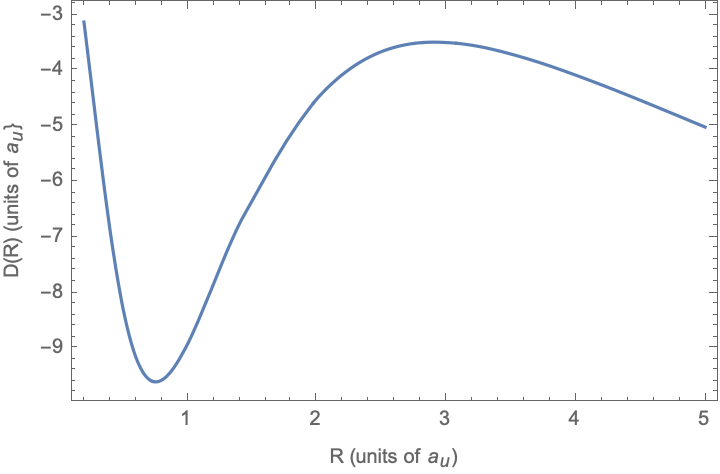
\includegraphics{DR.png}

WE then use transition dipole values to compute the cross section. 


\subsection{Result and discussion}


The Mathematica code used for calculation is shown n appendix E.
